\section{Liên trường Sở GD\&ĐT Hà Tĩnh, Lần 1, năm học 25-26}
\vspace{-0.5cm}
\Opensolutionfile{ans}[ans/ans-26-2-HaTinh-LienTruong-L1]
\caulc

\begin{ex}%[Thi thử L1, Liên Trường Hà Tĩnh, 2025-2026]%[Minh Trường,  Dự án 26-2-DuAnDeTHPT-2025-2026]%[2D1N3-1]
	Tìm giá trị lớn nhất của hàm số $y=\dfrac{2x+3}{x-1}$ trên đoạn $[2;4]$.
	\choice
	{$8$}
	{$\dfrac{9}{2}$}
	{\True $7$}
	{$\dfrac{11}{3}$}
	\loigiai{
		Tập xác định $\mathscr{D}=\mathbb{R}\setminus\{1\}$.\\
		Ta có $y'=\dfrac{-5}{(x-1)^2} < 0$, $\forall x \neq 1$.\\
		Hàm số nghịch biến trên khoảng $(1;+\infty) \Rightarrow$ hàm số nghịch biến trên $[2;4]$.\\
		Do đó $\max\limits_{[2;4]} y = y(2) = \dfrac{2\cdot 2+3}{2-1} = 7$.
	}
\end{ex}

\begin{ex}%%[Thi thử L1, Liên Trường Hà Tĩnh, 2025-2026]%[Minh Trường,  Dự án 26-2-DuAnDeTHPT-2025-2026]%[2D1H3-2]
	Giá trị lớn nhất của hàm số $y=3\sin 2x - 1$ là
	\choice
	{\True $2$}
	{$5$}
	{$4$}
	{$3$}
	\loigiai{
		Ta có $$-1 \le \sin 2x \le 1 \Rightarrow -3 \le 3\sin 2x \le 3 \Rightarrow -4 \le 3\sin 2x - 1 \le 2 \Rightarrow -4 \le y \le 2.$$
		Dấu bằng có thể xảy ra.\\
		Vậy giá trị lớn nhất của hàm số là $2$.
	}
\end{ex}

\begin{ex}%%[Thi thử L1, Liên Trường Hà Tĩnh, 2025-2026]%[Minh Trường,  Dự án 26-2-DuAnDeTHPT-2025-2026]%[1D2H2-3]
	Cho cấp số cộng $(u_n)$ có $u_1=2$, $u_5=14$. Tính $u_4$.
	\choice
	{$8$}
	{$7$}
	{$14$}
	{\True $11$}
	\loigiai{
		Ta có $$u_5 = u_1 + 4d \Rightarrow 2+4d=14 \Rightarrow d=3.$$
		Khi đó $$u_4 = u_1 + 3d = 2+3\cdot 3 = 11.$$
	}
\end{ex}

\begin{ex}%%[Thi thử L1, Liên Trường Hà Tĩnh, 2025-2026]%[Minh Trường,  Dự án 26-2-DuAnDeTHPT-2025-2026]%[2H2H1-3]
	\immini{
		Cho hình lập phương $ABCD.A'B'C'D'$ cạnh bằng $4$. Tính tích vô hướng $\vec{AC'} \cdot \vec{BC}$.
		\choice
		{$8\sqrt{3}$}
		{$16\sqrt{3}$}
		{\True $16$}
		{$0$}
	}{
		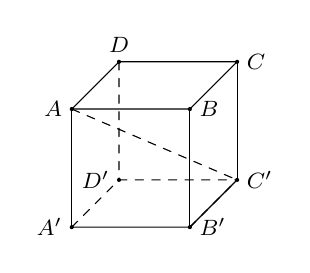
\begin{tikzpicture}[scale=0.5, font=\footnotesize, line join=round, line cap=round, >=stealth]
			\coordinate (A') at (0,0);
			\coordinate (B') at (3,0);
			\coordinate (D') at (1.2,1.2);
			\coordinate (C') at (4.2,1.2);
			\coordinate (A) at (0,3);
			\coordinate (B) at (3,3);
			\coordinate (D) at (1.2,4.2);
			\coordinate (C) at (4.2,4.2);
			\draw (A)--(B)--(C)--(D)--cycle;
			\draw (A')--(B')--(C');
			\draw (A)--(A') (B)--(B') (C)--(C');
			\draw[dashed] (A')--(D')--(C') (D)--(D');
			\draw[dashed] (A)--(C') (B')--(C');
			\fill (A) circle (1.5pt) node[left] {$A$};
			\fill (B) circle (1.5pt) node[right] {$B$};
			\fill (C) circle (1.5pt) node[right] {$C$};
			\fill (D) circle (1.5pt) node[above] {$D$};
			\fill (A') circle (1.5pt) node[left] {$A'$};
			\fill (B') circle (1.5pt) node[right] {$B'$};
			\fill (C') circle (1.5pt) node[right] {$C'$};
			\fill (D') circle (1.5pt) node[left] {$D'$};
		\end{tikzpicture}
	}
	\loigiai{
		Ta có $$\vec{AC'} \cdot \vec{BC} = \vec{AC'} \cdot \vec{B'C'} = \left|\vec{AC'}\right| \cdot \left|\vec{B'C'}\right| \cdot \cos\left(\vec{AC'}, \vec{B'C'}\right) = AC' \cdot B'C' \cdot \cos \widehat{AC'B'}.$$
		Xét tam giác $AB'C'$ có
		$$\cos \widehat{AC'B'} = \dfrac{AC'^2 + B'C'^2 - AB'^2}{2 \cdot AC' \cdot B'C'} = \dfrac{(4\sqrt{3})^2 + 4^2 - (4\sqrt{2})^2}{2 \cdot 4\sqrt{3} \cdot 4} = \dfrac{\sqrt{3}}{3}.$$
		Vậy $$\vec{AC'} \cdot \vec{BC} = 4\sqrt{3} \cdot 4 \cdot \dfrac{\sqrt{3}}{3} = 16.$$
	}
\end{ex}

\begin{ex}%%[Thi thử L1, Liên Trường Hà Tĩnh, 2025-2026]%[Minh Trường,  Dự án 26-2-DuAnDeTHPT-2025-2026]%[2D1N4-1]
	\impicinpar{
		Hàm số $y=f(x)$ có đồ thị như hình dưới đây.
		Đồ thị hàm số đã cho có đường tiệm cận ngang là
		\choice
		{$x=2$}
		{$x=1$}
		{\True $y=1$}
		{$y=2$}
	}{
		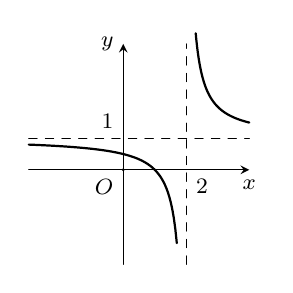
\begin{tikzpicture}[scale=0.4, font=\footnotesize, line join=round, line cap=round, >=stealth]
			\draw[->] (-3,0) -- (4,0) node[below] {$x$};
			\draw[->] (0,-3) -- (0,4) node[left] {$y$};
			\fill (0,0) circle (1.5pt) node[below left] {$O$};
			\draw[dashed] (-3,1) --(0,1)node[above left] {$1$}-- (4,1);
			\draw[dashed] (2,-3)--(2,0)node[below right] {$2$} -- (2,4);
			\draw[thick, domain=-3:1.7, samples=100] plot (\x, {1 + 1/(\x-2)});
			\draw[thick, domain=2.3:4, samples=100] plot (\x, {1 + 1/(\x-2)});
		\end{tikzpicture}
	}
	\loigiai{
		Đồ thị hàm số đã cho có đường tiệm cận ngang là $y=1$.
	}
\end{ex}

\begin{ex}%%[Thi thử L1, Liên Trường Hà Tĩnh, 2025-2026]%[Minh Trường,  Dự án 26-2-DuAnDeTHPT-2025-2026]%[2D2N1-2]
	Cho $0<a \neq 1$, $b>0$. Biết $\log_a b = 3$, tính $\log_a (ab)$.
	\choice
	{$3$}
	{\True $4$}
	{$\dfrac{1}{3}$}
	{$5$}
	\loigiai{
		Ta có $$\log_a (ab) = \log_a a + \log_a b = 1 + 3 = 4.$$
	}
\end{ex}

\begin{ex}%%[Thi thử L1, Liên Trường Hà Tĩnh, 2025-2026]%[Minh Trường,  Dự án 26-2-DuAnDeTHPT-2025-2026]%[2D1H5-3]
	\immini{
		Cho hàm số $f(x)=ax^3+bx^2+cx+d$ có đồ thị như hình bên.
		Số nghiệm dương của phương trình $2f(x)-3=0$ là
		\choice
		{$1$}
		{$0$}
		{$3$}
		{\True $2$}
	}{
		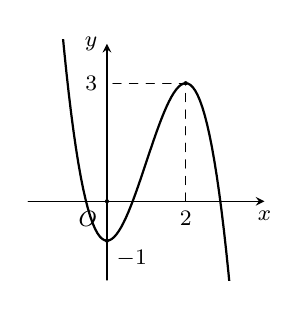
\begin{tikzpicture}[scale=0.5, font=\footnotesize, line join=round, line cap=round, >=stealth]
			\draw[->] (-2,0) -- (4,0) node[below] {$x$};
			\draw[->] (0,-2) -- (0,4) node[left] {$y$};
			\fill (0,0) circle (1.5pt) node[below left] {$O$};
			\draw[dashed] (2,0) node[below] {$2$} -- (2,3) -- (0,3) node[left] {$3$};
			\clip (-2,-2) rectangle (4.1,4.1);
			\draw[thick, domain=-2:4, samples=100] plot (\x, {-(\x)^3 +3*(\x)^2 - 1});
			\fill (2,3) circle (1.5pt);
			\fill (0,-1) circle (1.5pt) node[below right] {$-1$};
		\end{tikzpicture}
	}
	\loigiai{
		\immini
		{
			Phương trình $$2f(x)-3=0 \Leftrightarrow f(x)=\dfrac{3}{2}.$$
			Đường thẳng $y=\dfrac{3}{2}$ cắt đồ thị hàm số đã cho tại $2$ điểm có hoành độ dương.\\
			Vậy phương trình $2f(x)-3=0$ có $2$ nghiệm dương phân biệt.
		}
		{
			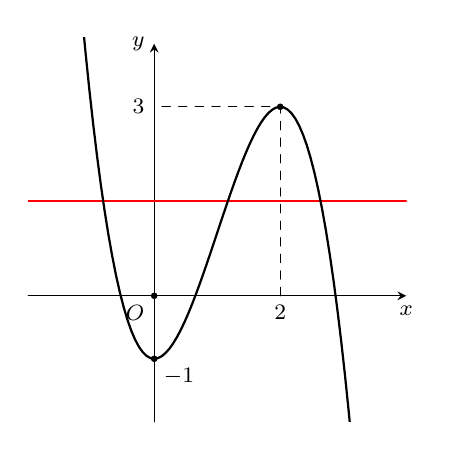
\begin{tikzpicture}[scale=0.8, font=\footnotesize, line join=round, line cap=round, >=stealth]
				\draw[->] (-2,0) -- (4,0) node[below] {$x$};
				\draw[->] (0,-2) -- (0,4) node[left] {$y$};
				\fill (0,0) circle (1.5pt) node[below left] {$O$};
				\draw[dashed] (2,0) node[below] {$2$} -- (2,3) -- (0,3) node[left] {$3$};
				\clip (-2,-2) rectangle (4.1,4.1);
				\draw[thick, red] (-2,1.5) -- (4,1.5);
				\draw[thick, domain=-2:4, samples=100] plot (\x, {-(\x)^3 +3*(\x)^2 - 1});
				\fill (2,3) circle (1.5pt);
				\fill (0,-1) circle (1.5pt) node[below right] {$-1$};
			\end{tikzpicture}
		}
	}
\end{ex}

\begin{ex}%%[Thi thử L1, Liên Trường Hà Tĩnh, 2025-2026]%[Minh Trường,  Dự án 26-2-DuAnDeTHPT-2025-2026]%[1H4H2-4]
		Cho hình tứ diện $ABCD$. Gọi $M$ là trọng tâm tam giác $BCD$. Đường thẳng qua $M$ song song với $AB$ cắt mặt phẳng $(ACD)$ tại $N$. Tính tỉ số $\dfrac{MN}{AB}$.
		\choice
		{$\dfrac{3}{4}$}
		{$\dfrac{2}{3}$}
		{\True $\dfrac{1}{3}$}
		{$\dfrac{1}{2}$}
	\loigiai{
		\immini
		{
			Gọi $I$ là trung điểm của $CD$, khi đó $M \in (ABI)$.\\
			Dựng $MN \parallel AB$ với $N \in AI$ mà $AI \subset (ACD)$ nên $N \in (ACD)$.\\
			Xét tam giác $ABI$ có
			$\heva{ & MN \parallel AB \\ & \dfrac{MI}{BI}=\dfrac{1}{3}} \Rightarrow \dfrac{MN}{AB}=\dfrac{1}{3}$.
		}
		{
			\begin{tikzpicture}[declare function={a=4;c=2;d=4;goc=-60;}, font=\footnotesize, line join=round, line cap=round, >=stealth]
				\coordinate (B) at (0,0);
				\coordinate (D) at (d,0);
				\coordinate (C) at (goc:c);
				\coordinate (A) at (60:a);
				\coordinate (I) at ($(C)!0.5!(D)$);
				\coordinate (M) at ($(B)!2/3!(I)$);
				\coordinate (N) at ($(A)!2/3!(I)$);
				\draw (A)--(B)--(C)--(D)--(A)--(C);
				\draw[dashed] (B)--(D) (A)--(I) (B)--(I) (M)--(N);
				\foreach \x/\g in {A/90,B/180,C/-90,D/0,M/-90,N/60,I/-45}
			\fill[black] 	(\x) circle (1pt)
			($(\g:3mm)+(\x)$) node {$\x$};
			\end{tikzpicture}
		}
	}
\end{ex}

\begin{ex}%%[Thi thử L1, Liên Trường Hà Tĩnh, 2025-2026]%[Minh Trường,  Dự án 26-2-DuAnDeTHPT-2025-2026]%[2D1N2-2]
	Cho hàm số $y=f(x)$ có bảng biến thiên như sau:
	\begin{center}
		
\begin{tikzpicture}
			\tkzTabInit[nocadre=false,lgt=1.2,espcl=2.5,deltacl=0.6]
			{$x$ / 0.6, $y'$ / 0.6, $y$ / 2}
			{$-\infty$, $-7$, $-4$, $+\infty$}
			\tkzTabLine{ , -, 0, +, 0, -, }
			\tkzTabVar{+/ $+\infty$, -/ $-6$, +/ $-3$, -/ $-\infty$}
		\end{tikzpicture}
	\end{center}
	Giá trị cực đại của hàm số $y=f(x)$ là
	\choice
	{\True $y=-3$}
	{$y=-6$}
	{$x=-7$}
	{$x=-4$}
	\loigiai{
		Dựa vào bảng biến thiên, giá trị cực đại của hàm số $y=f(x)$ là $y_\text{CĐ}=-3$.
	}
\end{ex}

\begin{ex}%%[Thi thử L1, Liên Trường Hà Tĩnh, 2025-2026]%[Minh Trường,  Dự án 26-2-DuAnDeTHPT-2025-2026]%[2D1H1-1]
	Hàm số $y=\log_2(x^2-2x)$ nghịch biến trên khoảng
	\choice
	{$(-\infty;1)$}
	{$(0;1)$}
	{\True $(-1;0)$}
	{$(2;+\infty)$}
	\loigiai{
		Tập xác định $\mathscr{D}=(-\infty;0) \cup (2;+\infty)$.\\
		Ta có $y'=\dfrac{(x^2-2x)'}{(x^2-2x)\ln 2}=\dfrac{2x-2}{(x^2-2x)\ln 2}$.\\
		Xét $y'=0 \Leftrightarrow 2x-2=0 \Leftrightarrow x=1 \notin \mathscr{D}$.\\
		Bảng biến thiên:
		\begin{center}
				\begin{tikzpicture}[yscale=1,xscale=1.5]
				\def\c{7} % số cột
				\def\d{4} % số dòng
				\foreach \x in {0,...,\c}{
					\foreach \y in {0,...,\d}
					\path[yscale=-1] (\x,\y) node[minimum size=1cm] (\x\y) {};
				}
				\fill[pattern=north east lines] (31.north) rectangle (54.south);
				\draw[shift={(-0.5,0.5)}] 
				(0,0) rectangle (\c+1, -\d-1) % Khung ngoài
				(0,-1) -- (\c+1, -1)          % Đường dưới x
				(0,-2) -- (\c+1, -2)          % Đường dưới y'
				(1,0) -- (1, -\d-1);          % Đường dọc sau cột tiêu đề
				\path[yscale=-1]
				(00) node {$x$}
				(01) node {$y'$}
				(03) node {$y$}
				(10) node {$-\infty$} (30) node {$0$} (40) node {$1$} (50) node {$2$} (70) node {$+\infty$}
				(21) node {$-$} (61) node {$+$}
				(12) node (y1) {$+\infty$}
				(72) node (y2) {$+\infty$};
				\node[anchor=east] at (34) {$0$};
				\node[anchor=west] at (54) {$2$};
				\draw[->, >=stealth] (y1) -- (34.west);
				\draw[->, >=stealth] (54.east) -- (y2);
				\draw[double, thick] (31.north) -- (34.south);
				\draw[double, thick] (51.north) -- (54.south);
			\end{tikzpicture}
		\end{center}
		Vậy hàm số đã cho nghịch biến trên khoảng $(-\infty;0)$ nên cũng nghịch biến trên $(-1;0)$.
	}
\end{ex}

\begin{ex}%%[Thi thử L1, Liên Trường Hà Tĩnh, 2025-2026]%[Minh Trường,  Dự án 26-2-DuAnDeTHPT-2025-2026]%[2D1H4-1]
	Đường tiệm cận xiên của đồ thị hàm số $y=x+4+\dfrac{x-1}{x-2}$ là:
	\choice
	{$y=x+4$}
	{$x=-2$}
	{\True $y=x+5$}
	{$y=x+3$}
	\loigiai{
		Ta có 
		$y = f(x) = x+4 + \dfrac{x-1}{x-2} = x+5 + \dfrac{1}{x-2}.$\\
		Vì $\lim\limits_{x \to \pm\infty} [f(x) - (x+5)] = \lim\limits_{x \to \pm\infty} \dfrac{1}{x-2} = 0$
		nên đường thẳng $y = x+5$ là đường tiệm cận xiên của đồ thị hàm số.
		}
\end{ex}

\begin{ex}%%[Thi thử L1, Liên Trường Hà Tĩnh, 2025-2026]%[Minh Trường,  Dự án 26-2-DuAnDeTHPT-2025-2026]%[1D5H2-2]
	Cho mẫu số liệu ghép nhóm có bảng tần số như sau:
	\begin{center}
		\begin{tabular}{|c|c|c|c|c|c|}
			\hline
			Nhóm & $[16;21)$ & $[21;26)$ & $[26;31)$ & $[31;36)$ & $[36;41)$ \\
			\hline
			Tần số & $4$ & $6$ & $8$ & $18$ & $4$ \\
			\hline
		\end{tabular}
	\end{center}
	Tính số trung vị của mẫu số liệu trên (làm tròn đến hàng phần mười).
	\choice
	{\True $31{,}6$}
	{$31{,}5$}
	{$30{,}6$}
	{$30{,}5$}
	\loigiai{
		Cỡ mẫu: $n = 4 + 6 + 8 + 18 + 4 = 40$.\\
		Trung vị $M_e$ thuộc nhóm thứ $k$ sao cho tần số tích lũy $cf_{k-1} < \dfrac{n}{2} = 20 \le cf_k$.\\
		Ta có: $cf_1=4, cf_2=10, cf_3=18, cf_4=36$.\\
		Vì $18 < 20 \le 36$ nên trung vị thuộc nhóm $[31;36)$.\\
		Áp dụng công thức trung vị: $M_e = L + \dfrac{\frac{n}{2} - cf_{k-1}}{f_k} \cdot w$.\\
		Trong đó $L=31, cf_{k-1}=18, f_k=18, w=5$.\\
		Ta có
		$M_e = 31 + \dfrac{20 - 18}{18} \cdot 5 = 31 + \dfrac{10}{18} \approx 31{,}6.$
	}
\end{ex}

\Closesolutionfile{ans}

\cauds
\Opensolutionfile{ans}[ans/ans-26-2-HaTinh-Lientruong-L1-DS]

\begin{ex}%%[Thi thử L1, Liên Trường Hà Tĩnh, 2025-2026]%[Minh Trường,  Dự án 26-2-DuAnDeTHPT-2025-2026]%[0D0V2-3]
	Một nhóm $12$ bạn học sinh đặt mua $12$ vé kề nhau trong một hàng có $12$ ghế để xem bộ phim ``Mưa Đỏ''. Tuy nhiên, đến hôm đi xem phim thì $3$ bạn bận đột xuất nên chỉ có $9$ bạn gồm $4$ bạn nam và $5$ bạn nữ đi xem phim. Nhân viên rạp chiếu phim sắp xếp ngẫu nhiên cho $9$ bạn vào $9$ trong $12$ hàng ghế đã mua (mỗi bạn một ghế).
	\choiceTF
	{\True Số cách sắp xếp $9$ bạn là $79833600$}
	{Xác suất để $9$ bạn ngồi cạnh nhau là $\dfrac{1}{220}$}
	{\True Xác suất để không có hai ghế trống cạnh nhau là $\dfrac{6}{11}$}
	{\True Xác suất để không có hai bạn nam nào ngồi cạnh nhau là $\dfrac{14}{55}$}
	\loigiai{
		\begin{itemchoice}
			\itemch Số cách sắp xếp $9$ bạn vào $12$ ghế là $\mathrm{A}_{12}^{9}=79833600$ cách.
			\itemch Giả sử ta đánh số ghế đã đặt trước từ $1$ đến $12$.\\
			Trường hợp 1: Xếp $9$ bạn ngồi ghế từ số $1$ đến $9$ có $9!$ cách.\\
			Trường hợp 2: Xếp $9$ bạn ngồi ghế từ số $2$ đến $10$ có $9!$ cách.\\
			Tương tự với trường hợp ngồi từ ghế số $3$ đến $11$ và từ ghế số $4$ đến $12$.\\
			Do đó số cách xếp $9$ bạn ngồi cạnh nhau là $4\cdot 9!$ cách.\\
			Xác suất để $9$ bạn ngồi cạnh nhau là $\dfrac{4\cdot 9!}{\mathrm{A}_{12}^{9}}=\dfrac{1}{55}$.
			\itemch Vì có $3$ bạn bận đột xuất nên số ghế trống là $3$ ghế.\\
			Số cách xếp chỗ để không có hai ghế trống cạnh nhau là $9!\cdot \mathrm{C}_{10}^{3}$.\\
			Xác suất để không có hai ghế trống cạnh nhau là $\dfrac{9!\cdot \mathrm{C}_{10}^{3}}{\mathrm{A}_{12}^{9}}=\dfrac{6}{11}$.
			\itemch Xếp $5$ ghế ngồi của bạn nữ và $3$ ghế trống thành $1$ hàng ngang, ta thấy có $9$ khoảng trống (tính cả $2$ đầu).\\
			Khi đó: Số cách xếp $4$ bạn nam vào $9$ chỗ ngồi là $\mathrm{A}_{9}^{4}$ cách.\\
			Vì vai trò của ghế trống là như nhau nên số cách chọn $3$ ghế trống là $\mathrm{C}_{8}^{3}$ cách.\\
			Số cách xếp $5$ bạn nữ vào $5$ ghế còn lại là $5!$ cách.\\
			Xác suất để không có hai bạn nam nào ngồi cạnh nhau là $\dfrac{\mathrm{A}_{9}^{4}\cdot \mathrm{C}_{8}^{3}\cdot 5!}{\mathrm{A}_{12}^{9}}=\dfrac{14}{55}$.
		\end{itemchoice}
	}
\end{ex}

\begin{ex}%%[Thi thử L1, Liên Trường Hà Tĩnh, 2025-2026]%[Minh Trường,  Dự án 26-2-DuAnDeTHPT-2025-2026]%[2D1V3-6]
	Bác Bình dự định làm một bể cá bằng kính cường lực dạng hình hộp chữ nhật không nắp. Bể có thể tích $3\text{ m}^3$ và có chiều dài gấp đôi chiều rộng. Chi phí làm bể gồm hai phần: phần làm đáy bể là $500$ ngàn đồng trên $1\text{ m}^2$ và phần làm mặt xung quanh là $400$ ngàn đồng trên $1\text{ m}^2$. Chi phí vận hành bể cá trong một tháng là $400$ ngàn đồng.
	\choiceTF
	{\True Chi phí vận hành bể cá trong một năm là $4{,}8$ triệu đồng}
	{Nếu chiều rộng của bể là $1\text{ m}$ thì chiều cao của bể là $3\text{ m}$}
	{\True Nếu chiều rộng của bể là $x (\text{m})$ thì diện tích xung quanh của bể là $\dfrac{9}{x} (\text{m}^2)$}
	{\True Chi phí ít nhất để làm bể là $4{,}44$ triệu đồng (làm tròn đến hàng phần trăm)}
	\loigiai{
		\begin{itemchoice}
			\itemch Chi phí vận hành bể trong $1$ năm là $400 \cdot 12 = 4800$ (nghìn đồng) hay $4{,}8$ triệu đồng.
			\itemch Vì chiều dài gấp đôi chiều rộng nên chiều rộng của bể là $1\text{ m}$ thì chiều dài là $2\text{ m}$. Thể tích là $3\text{ m}^3$ nên chiều cao của bể là $3 / (1 \cdot 2) = 1{,}5\text{ m}$.
			\itemch Giả sử chiều rộng của bể là $x$ $(\text{m}, x>0)$. Khi đó chiều dài của bể là $2x (\text{m})$.\\
			Chiều cao của bể là $\dfrac{3}{x \cdot 2x} = \dfrac{3}{2x^2}$.\\
			Diện tích xung quanh của bể là $(x+2x) \cdot 2 \cdot \dfrac{3}{2x^2} = \dfrac{9}{x} (\text{m}^2)$.
			\itemch Diện tích đáy bể là $2x^2 (\text{m}^2)$.\\
			Chi phí để làm bể là $500 \cdot 2x^2 + 400 \cdot \dfrac{9}{x} = 1000x^2 + \dfrac{3600}{x}$ (nghìn đồng).\\
			Đặt $y=f(x)=1000x^2+\dfrac{3600}{x}$ với $x>0$.\\
			Ta có $f'(x)=2000x-\dfrac{3600}{x^2}$. Xét $f'(x)=0 \Leftrightarrow x=\sqrt[3]{1{,}8}$.\\
			Bảng biến thiên hàm số:
			\begin{center}
				
\begin{tikzpicture}
					\tkzTabInit[nocadre=false, lgt=1, espcl=2.5, deltacl=0.6]
					{$x$ /0.6, $y'$ /0.6, $y$ /2} 
					{$0$, $\sqrt[3]{1{,}8}$, $+\infty$} 
					\tkzTabLine{ , - , 0 , + , }
					\tkzTabVar{+ / $+\infty$, - / $4439$, + / $+\infty$}
				\end{tikzpicture}
			\end{center}
			Ta thấy $f(x)$ đạt giá trị nhỏ nhất tại $x=\sqrt[3]{1{,}8}$ với $f(\sqrt[3]{1{,}8}) \approx 4439$ (nghìn đồng).\\
			Vậy chi phí ít nhất để làm bể là $4{,}44$ triệu đồng.
		\end{itemchoice}
	}
\end{ex}

\begin{ex}%%[Thi thử L1, Liên Trường Hà Tĩnh, 2025-2026]%[Minh Trường,  Dự án 26-2-DuAnDeTHPT-2025-2026]%[2D1V5-5]
	\immini
	{
			Cho hàm số $y=f(x)=\dfrac{ax+b}{x+c}$ có giá trị lớn nhất trên đoạn $[3;4]$ bằng $7$ và có đồ thị $y=f'(x)$ như hình vẽ (đồ thị hàm số $f'(x)$ có tiệm cận đứng $x=2$ và nhận trục hoành làm tiệm cận ngang).
		\choiceTF
		{\True Đồ thị $y=f'(x)$ có đường tiệm cận đứng là $x=2$}
		{\True Hàm số $f(x)$ nghịch biến trên khoảng $(2;+\infty)$}
		{$3b+2c=-2$}
		{Giá trị nhỏ nhất của hàm số $f(x)$ trên đoạn $[3;4]$ bằng $6$}
	}
	{
		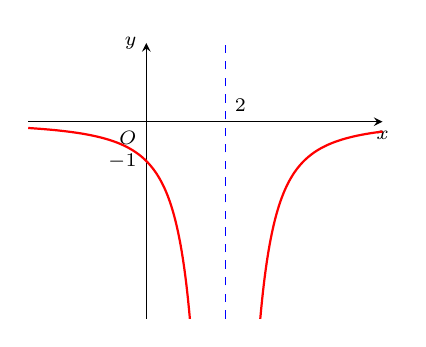
\begin{tikzpicture}[>=stealth,x=1cm,y=1cm,scale=0.5,declare function={xmin=-3;xmax=6;ymin=-5;ymax=2;can=2;}]
			\draw[->] (xmin,0) -- (xmax,0) node[below] {\scriptsize $x$};
			\draw[->] (0,ymin) -- (0,ymax) node[left] {\scriptsize $y$};
			\draw 
			(0,0) node[below left]{\scriptsize $O$}
			(2,0) node[above right]{\scriptsize $2$}
			(0,-1) node[left]{\scriptsize $-1$}
			;
			\draw[dashed,blue] (can,ymin) -- (can,ymax); 
			\clip (xmin,ymin) rectangle (xmax+0.1,ymax+0.1);
			\draw[thick,color=red,samples=150,smooth,domain=xmin:1.3] plot(\x,{-4/pow(\x-2,2)}); 
			\draw[thick,color=red,samples=150,smooth,domain=2.7:xmax] plot(\x,{-4/pow(\x-2,2)}); 
		\end{tikzpicture}
	}

	\loigiai{
		\begin{itemchoice}
			\itemch Từ đồ thị hàm số $y=f'(x)$, đường tiệm cận đứng là $x=2$.
			\itemch Trên khoảng $(2;+\infty)$, đồ thị $y=f'(x)$ nằm dưới trục hoành, nên $f'(x) < 0$, $\forall x \in (2;+\infty)$ nên hàm số $y=f(x)$ nghịch biến trên khoảng $(2;+\infty)$.
			\itemch Ta có $y=f'(x)=\dfrac{ac-b}{(x+c)^2}$.\\
			Từ đồ thị $f'(x)$ có tiệm cận đứng $x=2 \Rightarrow -c=2 \Leftrightarrow c=-2$.\\
			Mặt khác hàm số nghịch biến trên khoảng $(2;+\infty)$ nên trên đoạn $[3;4]$ hàm số cũng nghịch biến.\\
			Suy ra $\max\limits_{[3;4]} f(x) = f(3) = 7 \Leftrightarrow \dfrac{3a+b}{3+c} = 7 \Leftrightarrow 3a+b=7(3-2)=7$.\\
			Lại có từ đồ thị $f'(0)=-1 \Leftrightarrow \dfrac{ac-b}{c^2}=-1 \Leftrightarrow \dfrac{-2a-b}{4}=-1 \Leftrightarrow 2a+b=4$.\\
			Giải hệ ta được $a=3, b=-2$.\\
			Nên $3b+2c=3(-2)+2(-2)=-10 \neq -2$.
			\itemch Vì trên đoạn $[3;4]$ hàm số nghịch biến nên $\min\limits_{[3;4]} f(x) = f(4) = \dfrac{3\cdot 4 - 2}{4 - 2} = 5$.
		\end{itemchoice}
	}
\end{ex}

\begin{ex}%%[Thi thử L1, Liên Trường Hà Tĩnh, 2025-2026]%[Minh Trường,  Dự án 26-2-DuAnDeTHPT-2025-2026]%[2H2V2-6]
	Trong không gian với hệ tọa độ $Oxyz$ (đơn vị trên mỗi trục là $10\text{ km}$), hai khinh khí cầu A và B bay với vectơ vận tốc lần lượt là $\vec{v_a}=(1;2;0)$ và $\vec{v_b}=(-2;3;0)$ (đơn vị là $\text{km/giờ}$). Tại thời điểm $t=0$ vị trí của khinh khí cầu A là $M(5;4;2)$ và vị trí của khinh khí cầu B là $N(6;5;3)$. Hai khinh khí cầu sẽ bay trong $10$ giờ tiếp theo và dừng lại.
	\choiceTF
	{\True Sau $3$ giờ vị trí của khinh khí cầu A là $M'(8;10;2)$}
	{Khinh khí cầu B không bay qua vị trí $N'(0;14;3)$}
	{Khoảng cách giữa hai khinh khí cầu sau $3$ giờ là $9\text{ km}$}
	{\True Trong khoảng thời gian từ $t=0$ đến $t=10$ giờ, khoảng cách ngắn nhất giữa hai khinh khí cầu là $16{,}1\text{ km}$ (làm tròn đến hàng phần chục)}
	\loigiai{
		\begin{itemchoice}
			\itemch Giả sử sau $t$ giờ, vị trí máy bay A là $M'$, khi đó ta có $\vec{MM'} = t\vec{v_a} = (t;2t;0)$.\\
			Khi đó $M'(t+5; 2t+4; 2)$.\\
			Với $t=3 \Rightarrow M'(8;10;2)$.
			\itemch Giả sử sau $t$ giờ, vị trí máy bay B là $N'$, khi đó ta có $\vec{NN'} = t\vec{v_b} = (-2t;3t;0)$.\\
			Khi đó $N'(-2t+6; 3t+5; 3)$.\\
			Nếu khinh khí cầu B bay qua vị trí $N'(0;14;3)$ khi đó ta có $\heva{ & -2t+6=0 \\ & 3t+5=14 } \Leftrightarrow t=3$ (thỏa mãn).\\
			Vậy khinh khí cầu B có bay qua vị trí $N'(0;14;3)$.
			\itemch Sau $3$ giờ vị trí khinh khí cầu $B$ là $N'(0;14;3)$.\\
			Khoảng cách giữa hai khinh khí cầu trong không gian $Oxyz$ là $$M'N' = \sqrt{(0-8)^2+(14-10)^2+(3-2)^2} = \sqrt{81} = 9.$$
			Vì mỗi đơn vị trên trục là $10\text{ km}$ nên khoảng cách thực tế là $9 \cdot 10 = 90\text{ km}$.
			\itemch Gọi $t$ là thời điểm hai khinh khí cầu bay ($0 \le t \le 10$).\\
			Khi đó $M'(t+5; 2t+4; 2)$ và $N'(-2t+6; 3t+5; 3)$.\\
			Ta có 
			\allowdisplaybreaks
			\begin{eqnarray*}
				&&\vec{M'N'} = (-3t+1; t+1; 1)\\
				&\Rightarrow& M'N' = \sqrt{(-3t+1)^2+(t+1)^2+1} = \sqrt{10t^2-4t+3} = \sqrt{10\left(t-\dfrac{1}{5}\right)^2+\dfrac{13}{5}} \ge \sqrt{\dfrac{13}{5}}
			\end{eqnarray*}
			Suy ra $M'N'$ đạt giá trị nhỏ nhất là $\sqrt{\dfrac{13}{5}} \approx 1{,}61$ (đơn vị) ứng với $16{,}1\text{ km}$ khi $t=\dfrac{1}{5}$.
		\end{itemchoice}
	}
\end{ex}


\Closesolutionfile{ans}

\Opensolutionfile{ans}[ans/ans-26-2-HaTinh-Lientruong-L1-KQ]
\caukq


\begin{ex}%%[Thi thử L1, Liên Trường Hà Tĩnh, 2025-2026]%[Minh Trường,  Dự án 26-2-DuAnDeTHPT-2025-2026]%[2D1V3-6]
	Một doanh nghiệp sản xuất đồ gỗ nội thất cần mỗi ngày $5$ khối gỗ để làm các sản phẩm nội thất. Chi phí một lần vận chuyển gỗ từ cơ sở cung cấp gỗ đến nơi sản xuất của doanh nghiệp là $8$ triệu đồng, chi phí lưu kho tại doanh nghiệp của $1$ khối gỗ là $200$ ngàn đồng trên ngày. Mỗi lần vận chuyển, gỗ sẽ được đưa đến đầu ngày làm việc và lượng gỗ được vận chuyển vừa đủ cho doanh nghiệp sử dụng từ ngày hôm đó cho đến lần vận chuyển tiếp theo. Hỏi doanh nghiệp cần vận chuyển gỗ mấy ngày một lần để chi phí trung bình trong một ngày là nhỏ nhất?
	\shortans{4}
	\loigiai{
		Gọi $x$ (ngày) là số ngày giữa $2$ lần vận chuyển gỗ liên tiếp ($x \in \mathbb{N}^*$).\\
		Lượng gỗ mỗi lần nhập về là $5x$ khối.
		\begin{itemize}
			\item Chi phí vận chuyển trung bình mỗi ngày là $\dfrac{8000}{x}$ (ngàn đồng).
			\item Vì lượng gỗ được đưa đến đầu ngày và sử dụng vừa đủ cho đến lần vận chuyển tiếp theo nên lượng gỗ lưu trữ trung bình mỗi ngày là $\dfrac{5x+0}{2} = 2{,}5x$ (khối).
			\item Chi phí lưu trữ trung bình mỗi ngày là $2{,}5x \cdot 200 = 500x$ (ngàn đồng).
		\end{itemize}
		Tổng chi phí trung bình mỗi ngày là $C(x) = \dfrac{8000}{x} + 500x$ (ngàn đồng).\\
		Áp dụng bất đẳng thức Cô-si cho hai số dương, ta có:
		\begin{eqnarray*}
			C(x) = \dfrac{8000}{x} + 500x &\ge& 2\sqrt{\dfrac{8000}{x} \cdot 500x} = 2\sqrt{4\,000\,000} = 4000.
		\end{eqnarray*}
		Dấu bằng xảy ra khi và chỉ khi
		\begin{eqnarray*}
			\dfrac{8000}{x} = 500x &\Leftrightarrow& x^2 = 16 \\
			&\Leftrightarrow& x = 4 \text{ (do } x \in \mathbb{N}^*).
		\end{eqnarray*}
		Vậy doanh nghiệp cần vận chuyển gỗ $4$ ngày một lần để chi phí trung bình trong một ngày là nhỏ nhất.
	}
\end{ex}

\begin{ex}%%[Thi thử L1, Liên Trường Hà Tĩnh, 2025-2026]%[Minh Trường,  Dự án 26-2-DuAnDeTHPT-2025-2026]%[2H2V1-3]
	Trong không gian với hệ tọa độ $Oxyz$, cho hai điểm $A(6;5;-1)$, $B(4;-2;3)$. Tính số đo góc nhị diện $[A,Ox,B]$ theo đơn vị độ.
	\shortans{135}
	\loigiai{
		Gọi $A_1$, $B_1$ lần lượt là hình chiếu của $A(6;5;-1)$, $B(4;-2;3)$ lên mặt phẳng $(Oyz)$.\\
		Khi đó $A_1(0;5;-1)$, $B_1(0;-2;3)$.\\
		Góc nhị diện $[A,Ox,B]$ có số đo bằng góc giữa hai vectơ $\vec{OA_1}$ và $\vec{OB_1}$.\\
		Ta có $\vec{OA_1} = (0;5;-1)$, $\vec{OB_1} = (0;-2;3)$.
		\begin{eqnarray*}
			\cos\left(\vec{OA_1}, \vec{OB_1}\right) &=& \dfrac{\vec{OA_1} \cdot \vec{OB_1}}{\left|\vec{OA_1}\right| \cdot \left|\vec{OB_1}\right|} \\
			&=& \dfrac{5 \cdot (-2) + (-1) \cdot 3}{\sqrt{5^2 + (-1)^2} \cdot \sqrt{(-2)^2 + 3^2}} \\
			&=& -\dfrac{\sqrt{2}}{2}.
		\end{eqnarray*}
		Suy ra sđ $[A,Ox,B] = 135^{\circ}$.
	}
\end{ex}

\begin{ex}%%[Thi thử L1, Liên Trường Hà Tĩnh, 2025-2026]%[Minh Trường,  Dự án 26-2-DuAnDeTHPT-2025-2026]%[1D2V3-7]
	Anh Bảo vừa tốt nghiệp đại học và được nhận vào làm việc tại tập đoàn dược mỹ phẩm PBC với một trong hai phương án lương như sau:
	\begin{itemize}
		\item \textbf{Phương án 1:} Lương khởi điểm $10$ triệu đồng một tháng, cứ sau tròn $3$ năm thì tăng lương mỗi tháng $6$ triệu đồng so với mỗi tháng của $3$ năm trước đó.
		\item \textbf{Phương án 2:} Lương khởi điểm $10$ triệu đồng một tháng, cứ sau tròn $3$ năm thì tăng lương mỗi tháng $40\%$ so với mỗi tháng của $3$ năm trước đó.
	\end{itemize}
	Nếu anh Bảo kí hợp đồng làm việc $20$ năm thì sau $20$ năm đi làm, tổng tiền lương anh nhận được theo phương án $2$ nhiều hơn phương án $1$ bao nhiêu triệu đồng (làm tròn đến hàng đơn vị)?
	\shortans{1180}
	\loigiai{
		Trong $20$ năm làm việc, ta có $6$ chu kỳ $3$ năm và dư lại $2$ năm cuối ($24$ tháng).
		\begin{itemize}
			\item Số tiền nhận được sau $20$ năm đi làm nếu kí hợp đồng theo phương án 1 là
			\begin{eqnarray*}
				T_1 &=& 36 \cdot (10 + 16 + 22 + 28 + 34 + 40) + 24 \cdot 46 \\
				&=& 6504 \text{ (triệu đồng)}.
			\end{eqnarray*}
			\item Số tiền nhận được sau $20$ năm đi làm nếu kí hợp đồng theo phương án 2 là
			\begin{eqnarray*}
				T_2 &=& 36 \cdot 10 \cdot \dfrac{1 - 1{,}4^6}{1 - 1{,}4} + 24 \cdot 10 \cdot 1{,}4^6 \\
				&=& \dfrac{24011472}{3125} \approx 7683{,}67 \text{ (triệu đồng)}.
			\end{eqnarray*}
		\end{itemize}
		Số tiền chênh lệch giữa hai phương án là
		\begin{eqnarray*}
			\Delta T = T_2 - T_1 \approx 7683{,}67 - 6504 \approx 1180 \text{ (triệu đồng)}.
		\end{eqnarray*}
		Vậy sau $20$ năm, phương án $2$ nhận được nhiều hơn phương án $1$ khoảng $1180$ triệu đồng.
	}
\end{ex}

\begin{ex}%%[Thi thử L1, Liên Trường Hà Tĩnh, 2025-2026]%[Minh Trường,  Dự án 26-2-DuAnDeTHPT-2025-2026]%[1H8V5-3]
	\immini{Cho hình chóp $S.ABCD$ có đáy là hình vuông và $SA$ vuông góc với đáy, $SA = 3$, $AB = 2$. Tính khoảng cách từ điểm $C$ đến mặt phẳng $(SBD)$ (làm tròn đến hàng phần trăm).}{\begin{tikzpicture}[scale=0.8, font=\footnotesize, line join=round, line cap=round, >=stealth]
		\coordinate (A) at (0,0);
		\coordinate (B) at (-1,-1);
		\coordinate (D) at (3,0);
		\coordinate (C) at ($(B)+(D)-(A)$);
		\coordinate (S) at ($(A)+(0,2.5)$);
		\draw(S)--(B)--(C)--(S)--(D)--(C);
		\draw[dashed](S)--(A)--(B)--(D)--(A);
		\foreach \i/\g in {S/90,A/160,B/-90,C/-90,D/0}{\draw[fill=black](\i) circle (1.2pt) ($(\i)+(\g:3mm)$) node{$\i$};}
\end{tikzpicture}}
\shortans{1,28}
\loigiai{
	\immini{
		Gọi $O = AC \cap BD$. Vì $ABCD$ là hình vuông nên $O$ là trung điểm của $AC$.\\
		Ta có $\dfrac{\mathrm{d}(C, (SBD))}{\mathrm{d}(A, (SBD))} = \dfrac{OC}{OA} = 1$.\\
		Suy ra $\mathrm{d}(C,(SBD)) = \mathrm{d}(A,(SBD))$.\\
		Kẻ $AH \perp SO$ tại $H$.\\
		Vì $BD \perp AC$ và $BD \perp SA$ nên $BD \perp (SAC) \Rightarrow BD \perp AH$.\\
		Từ đó suy ra $AH \perp (SBD) \Rightarrow \mathrm{d}(A, (SBD)) = AH$.\\
		Xét tam giác $SAC$ vuông tại $A$, có $AC = 2\sqrt{2} \Rightarrow AO = \sqrt{2}$.\\
		Áp dụng hệ thức lượng trong tam giác vuông $SAO$ ta có\\
		$\dfrac{1}{AH^2} = \dfrac{1}{SA^2} + \dfrac{1}{AO^2} = \dfrac{1}{3^2} + \dfrac{1}{(\sqrt{2})^2} \Rightarrow AH = \dfrac{3\sqrt{22}}{11} \approx 1{,}28$.\\
		Vậy $\mathrm{d}(C,(SBD)) = AH \approx 1{,}28$.}{\begin{tikzpicture}[scale=1, font=\footnotesize, line join=round, line cap=round, >=stealth]
			\coordinate (A) at (0,0);
			\coordinate (B) at (-1,-1);
			\coordinate (D) at (3,0);
			\coordinate (C) at ($(B)+(D)-(A)$);
			\coordinate (S) at ($(A)+(0,3)$);
			\coordinate (O) at ($(A)!.5!(C)$);
			\coordinate (H) at ($(S)!.6!(O)$);
			\draw(S)--(B)--(C)--(S)--(D)--(C);
			\draw[dashed](S)--(A)--(B)--(D)--(A)--(C) (S)--(O) (A)--(H);
			\foreach \i/\g in {S/90,A/160,B/-90,C/-90,D/0,O/-90,H/0}{\draw[fill=black](\i) circle (1.2pt) ($(\i)+(\g:3mm)$) node{$\i$};}
			\draw pic[draw=black,angle radius=0.2cm] {right angle = O--H--A};
	\end{tikzpicture}}
}
\end{ex}


\begin{ex}%%[Thi thử L1, Liên Trường Hà Tĩnh, 2025-2026]%[Minh Trường,  Dự án 26-2-DuAnDeTHPT-2025-2026]%[2D1V3-6]
	Trong một buổi tập luyện của lính đặc công, một chiến sỹ cần phối hợp bơi và chạy bộ để từ điểm $A$ ở bờ sông bên này đến điểm $B$ về phía hạ lưu của bờ sông bên kia. Chiến sỹ dự định bơi thẳng từ điểm $A$ đến một điểm thuộc đoạn $HB$ sau đó chạy từ điểm đó về điểm $B$.
	\immini{
	 Biết $AH = 300$ m, $HB = 900$ m, vận tốc dòng nước là $1$ m/s, vận tốc bơi của chiến sỹ đối với nước là $1$ m/s và vận tốc chạy trên bờ của chiến sỹ là $3$ m/s. Hỏi chiến sỹ cần ít nhất bao nhiêu giây để hoàn thành kế hoạch trên? (làm tròn đến hàng đơn vị).}{	\begin{tikzpicture}[scale=1, font=\footnotesize, line join=round, line cap=round, >=stealth]
		\path (0,0) coordinate (A);
		\path (0,2.5) coordinate (H);
		\path (4,2.5) coordinate (C);
		\path (6,2.5) coordinate (B);
		\draw (-1,0) -- (3.5,0) node[below left] {Bờ}--(7,0);
		\draw (-1,2.5) -- (7,2.5);
		\draw[dashed] (-1,0.6) -- (7,0.6) 	(-1,1.2) -- (7,1.2) (-1,1.9) -- (7,1.9);
		\draw[->] (4,1.4) -- (5,1.4) node[midway, above=-1pt] {Nước};
		\draw (A) -- (H) (A) -- (C) (H) -- (B);
		\draw (0,2.3) -- (0.2,2.3) -- (0.2,2.5);
		\foreach \x in {A,H,C,B} \draw[fill=black] (\x) circle (1pt);
		\foreach \i/\g in {A/-90,B/90,C/90,H/90}{\draw[fill=black](\i) circle (1.2pt) ($(\i)+(\g:3mm)$) node{$\i$};}
\end{tikzpicture}}
\shortans{473}
\loigiai{
	\begin{center}
		\begin{tikzpicture}[scale=1, font=\footnotesize, line join=round, line cap=round, >=stealth]
			\path (0,0) coordinate (A);
			\path (0,3) coordinate (H);
			\path (1.5,3) coordinate (D);
			\path (4,3) coordinate (C);
			\path (8,3) coordinate (B);
			\draw (-1,0) -- (9,0);
			\draw (-1,3) -- (9,3);
			\path ($(A)!0.25!(D)$) coordinate (M);
			\path ($(M) + ($(B)-(C)$)$) coordinate (t);
			\path (intersection of A--C and M--t) coordinate (N); 
			\draw (A) -- (H) (A) -- (C) (A) -- (D);
			\draw[->] (A) -- (M);
			\draw[->] (M) -- (N);
			\draw[->](A) -- (N);
			\foreach \i/\g in {A/-90,B/90,C/90,D/90,H/90}{\draw[fill=black](\i) circle (1.2pt) ($(\i)+(\g:3mm)$) node{$\i$};}
			\foreach \i/\g in {M/130,N/-25}{\draw(\i) circle (0pt) ($(\i)+(\g:2.5mm)$) node{$\i$};}
			\draw pic[draw=black,angle radius=0.2cm] {right angle = A--H--C};
		\end{tikzpicture}
	\end{center}
	Gọi $\overrightarrow{AM}, \overrightarrow{MN}$ lần lượt là vectơ vận tốc bơi của chiến sỹ đối với nước và vectơ vận tốc dòng nước.\\
	Khi đó $\overrightarrow{AN} = \overrightarrow{AM} + \overrightarrow{MN}$ là vectơ vận tốc bơi của chiến sỹ đối với bờ.\\
	Gọi $C, D$ lần lượt là giao điểm của $AN, AM$ với $HB$ và $x = HD$ (đơn vị $\mathrm{m}$, $x \ge 0$).\\
	Thời gian bơi là $t_1 = \dfrac{AC}{AN} = \dfrac{AD}{AM} = \dfrac{\sqrt{x^2 + 300^2}}{1} = \sqrt{x^2 + 300^2}$.\\
	Ta có $\dfrac{DC}{MN} = \dfrac{AD}{AM} \Rightarrow DC = AD = \sqrt{x^2 + 300^2}$.\\
	Khi đó quãng đường chạy bộ là $CB = HB - HD - DC = 900 - x - \sqrt{x^2 + 300^2}$.\\
	Thời gian chạy bộ là $t_2 = \dfrac{CB}{3} = \dfrac{900 - x - \sqrt{x^2 + 300^2}}{3}$.\\
	Tổng thời gian thực hiện kế hoạch là:\\
	$f(x) = t_1 + t_2 = \sqrt{x^2 + 300^2} + \dfrac{900 - x - \sqrt{x^2 + 300^2}}{3} = \dfrac{2}{3}\sqrt{x^2 + 300^2} - \dfrac{x}{3} + 300$.\\
	Xét hàm số $f(x)$ trên $[0; 900]$, ta có $f'(x) = \dfrac{2x}{3\sqrt{x^2 + 300^2}} - \dfrac{1}{3}$.\\
	$f'(x) = 0 \Leftrightarrow 2x = \sqrt{x^2 + 300^2} \Leftrightarrow 4x^2 = x^2 + 300^2 \Leftrightarrow 3x^2 = 90\,000 \Leftrightarrow x = 100\sqrt{3}$.\\
	Giá trị nhỏ nhất của $f(x)$ đạt được tại $x = 100\sqrt{3}$, khi đó $f(100\sqrt{3}) = 200\sqrt{3} + 126{,}79 \approx 473{,}2$. \\
	Làm tròn đến hàng đơn vị ta được $473$ giây.
}
\end{ex}


\begin{ex}%%[Thi thử L1, Liên Trường Hà Tĩnh, 2025-2026]%[Minh Trường,  Dự án 26-2-DuAnDeTHPT-2025-2026]%[2D1V3-6]
	\immini{Một công viên nhỏ trong một khu dân cư có dạng hình chữ nhật với chiều rộng là $40$ m và chiều dài là $60$ m. Ban quản lý lát gạch phần đất dạng parabol và hình tròn bán kính $10$ m như hình vẽ. Phần còn lại sẽ trồng cỏ và cây xanh. Ban quản lý dự định làm một đoạn đường nhỏ nối hai phần lát gạch. Biết $AB = 20$ m, $OH = 30$ m, hỏi chiều dài ngắn nhất của đoạn đường đó là bao nhiêu mét (làm tròn đến hàng phần chục)?}{\begin{tikzpicture}[scale=0.6, font=\footnotesize, line join=round, line cap=round, >=stealth]
			\path (0,0) coordinate (A);
			\path (2,0) coordinate (B);
			\path (1,0) coordinate (H);
			\path (1,3) coordinate (O);
			\draw (0,0) -- (4,0) -- (4,6) -- (0,6) -- cycle;
			\draw[samples=100, domain=0:2] plot (\x, {-3*(\x-1)*(\x-1)+3});
			\draw (A) -- (B) (H) -- (O); 
			\path (3,5) coordinate (I);
			\draw (I) circle (1);
			\draw[fill=black] (3,5) circle (1pt); 
			\foreach \i/\g in {A/-90,B/-90,H/-90,O/90}{\draw[fill=black](\i) circle (1.2pt) ($(\i)+(\g:3mm)$) node{$\i$};}
			\draw pic[draw=black,angle radius=0.2cm] {right angle = O--H--B};
	\end{tikzpicture}}
	\shortans{17{,}7}
	\loigiai{
		\immini{
			Gắn hệ trục tọa độ như hình vẽ. Ta có $B(10; -30)$ và tâm hình tròn là $I(20; 20)$.\\
			Vì parabol có đỉnh là $O$ nên có phương trình dạng $y = ax^2 \quad (*)$.\\
			Thay tọa độ $B(10; -30)$ vào $(*)$ ta được: \[-30 = a \cdot 10^2 \Rightarrow a = -\dfrac{3}{10}.\]
			Gọi $M\left(x; -\dfrac{3x^2}{10}\right)$ là điểm thuộc parabol với $x \in [0; 10]$.\\
			Khoảng cách từ $M$ đến tâm $I$ của hình tròn là:\\
			$IM = \sqrt{(x - 20)^2 + \left(\dfrac{3}{10}x^2 + 20\right)^2}$.\\
			Sử dụng máy tính cầm tay hoặc khảo sát hàm số, ta tìm được giá trị nhỏ nhất của $IM$ xấp xỉ $27{,}7$ tại $x \approx 1{,}49$.\\
			Đoạn đường ngắn nhất nối từ parabol đến hình tròn là\\
			$d_{\min} = IM_{\min} - R$, với $R = 10$ là bán kính hình tròn.\\
			Vậy độ dài ngắn nhất của đoạn đường là $27{,}7 - 10 = 17{,}7$ m.}{\begin{tikzpicture}[scale=1, font=\footnotesize, line join=round, line cap=round, >=stealth]
				\draw[->] (-1.5,0)--(3.5,0) node[below]{$x$};
				\draw[->] (0,-3.5)--(0,3.5) node[left]{$y$};
				\path (-1,-3) coordinate (A);
				\path (1,-3) coordinate (B);
				\path (0,-3) coordinate (H);
				\path (0,0) coordinate (O);
				\draw (-1,-3)--(-1,0)node[below left]{$-10$} -- (-1,3)--(0,3)node[below right]{$30$} -- (3,3)--(3,0)node[below left]{$30$} -- (3,-3)--(0,-3)node[below left]{$-30$} -- cycle;
				\draw[samples=100, domain=-1:1] plot (\x, {-3*(\x)*(\x)});
				\path (2,2) coordinate (I);
				\draw[dashed](0,2) node[left]{$20$}--(I)--(2,0)node[below]{$20$} (B)--(1,0)node[above]{$10$};
				\draw (I) circle (1);
				\foreach \i/\g in {A/-90,B/-90,H/-45,O/45,I/45}{\draw[fill=black](\i) circle (1.2pt) ($(\i)+(\g:3mm)$) node{$\i$};}
				\draw pic[draw=black,angle radius=0.2cm] {right angle = O--H--B};
		\end{tikzpicture}}
	}
\end{ex}
\Closesolutionfile{ans}